\documentclass[chaptersright]{informeutn}
\usepackage{circuitikz}
\usepackage{amssymb}
\tikzset{every picture/.style={line width=0.75pt}} %set default line width to 0.75pt        

% Datos del informe
\materia{Electrónica Aplicada I}
\titulo{Trabajo Práctico 3}
\comision{3R2}
\autores{
          Gaston Grasso - 401892\\
          Franco Palombo - 401910\\
          Angelo Prieto - 401012}
\fecha{20/08/2025}

\begin{document}
  \maketitle
  \tableofcontents
  \setcounter{page}{1}
  \thispagestyle{plain}

\chapter{Introducción}

\chapter{Diseño para Máxima Excursión Simétrica}
En la Figura \ref{fig:amplificador} se muestra el circuito utilizado en el presente trabajo práctico. El mismo consiste
en un amplificador basado en un transistor BJT en configuración emisor común con 
polarización mediante divisor resistivo. Esta topología se caracteriza por permitir un punto de operación
estable frente a variaciones del $\beta$. 
El circuito incluye las resistencias $R_1$, $R_2$, $R_E$, $R_C$ y $R_L$, junto a capacitores de desacople y una fuente de 
alimentación $V_{CC}$. Algunos de estos valores fueron fijados por las consignas del trabajo.

\begin{figure}[!ht]
    \centering
    \begin{tikzpicture}
    	\node[npn](N1) at (9.25, 5.75){} node[anchor=west] at (N1.text){$Q1$};
    	\draw (7, 5) to[american resistor, l={$R_1$}] (7, 2.75);
    	\draw (7, 5.75) to[capacitor, l={$C_1$}] (3, 5.75);
    	\draw (7, 5.75) -- (8.41, 5.75);
    	\draw (9.25, 5) to[american resistor, l={$R_E$}] (9.25, 2.75);
    	\draw (3, 5.75) to[sinusoidal voltage source, l={$v_i$}] (3, 2.5);
    	\draw (7, 8.75) to[american resistor, l={$R_2$}, name=R1] (7, 6.5);
    	\draw (9.25, 8.77) to[american resistor, l={$R_c$}] (9.25, 6.52);
    	\draw (7, 5) -| (7, 6.5);
    	\draw (11, 5) to[capacitor, l={$C_E$}] (11, 2.75);
    	\draw (9.25, 5) -- (11, 5);
    	\draw (7, 8.75) -| (7, 9) -| (9.25, 8.77);
    	\draw (11, 2.75) |- (7, 2.5) -| (7, 2.75);
    	\draw (9.25, 2.75) -| (9.25, 2.5);
    	\draw (3, 2.5) -- (7, 2.5);
    	\draw (10.25, 6.5) to[capacitor, l={$C_2$}] (13, 6.5);
    	\draw (13.75, 5.5) to[american resistor, l={$R_L$}] (13.75, 3.25);
    	\draw (13.75, 6.5) -| (13.75, 5.5);
    	\draw (11, 2.5) -| (13.75, 3.25);
    	\node[vcc](N2) at (9.25, 9.75){} node[anchor=south] at (N2.text){$V_{CC}$};
    	\draw (9.25, 9) -| (9.25, 9.75);
    	\node[ground] at (9.25, 2){};
    	\draw (9.25, 2.5) -| (9.25, 2);
    	\draw (10.25, 6.5) -- (9.25, 6.5);
    	\draw (13, 6.5) -- (13.75, 6.5);
    \end{tikzpicture}
    \caption{amplificador emisor común.}
    \label{fig:amplificador}
\end{figure}

El objetivo de esta sección es establecer las condiciones de polarización en corriente continua de 
manera que el transistor opere en la región activa, garantizando linealidad en la 
amplificación de señales pequeñas. En particular, se busca ubicar el punto de operación $Q$ 
en la recta de carga de tal forma que la señal de salida pueda desplazarse con la mayor 
amplitud posible antes de alcanzar las regiones de saturación o corte.

Este criterio se conoce como polarización para máxima excursión simétrica (MES). Consiste 
en ajustar el punto de operación en el centro de las características de salida del transistor, 
de modo que la señal alterna pueda oscilar con igual margen hacia arriba y hacia abajo, 
evitando distorsiones. La Figura \ref{fig:gráfica-mes} ilustra este concepto, donde se observa el punto 
$Q_{MES}$, así como la comparación entre la recta de carga de continua y la de alterna.


\begin{figure}[!ht]
    \centering
    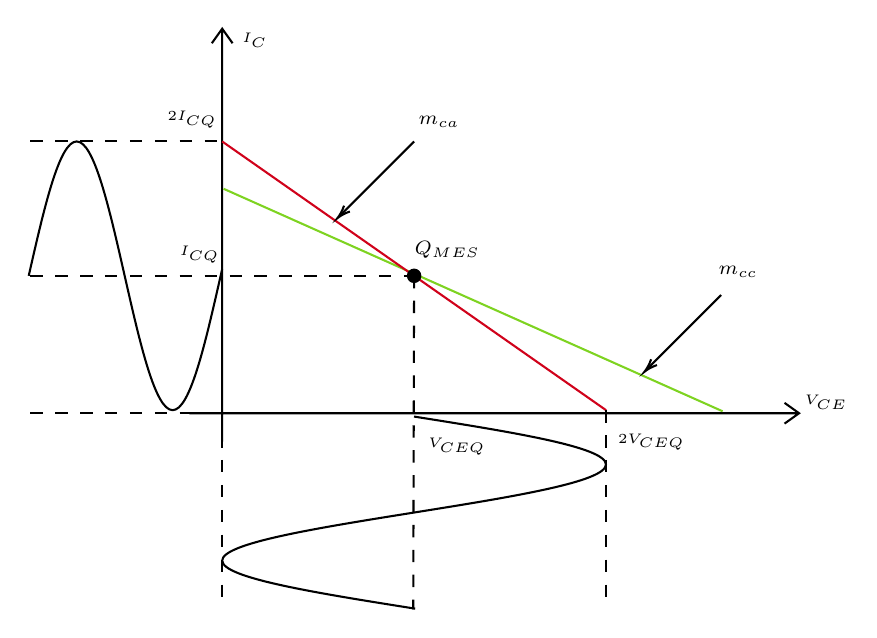
\begin{tikzpicture}[x=0.75pt,y=0.75pt,yscale=-1,xscale=1]
    %uncomment if require: \path (0,538); %set diagram left start at 0, and has height of 538
    
    %Shape: Axis 2D [id:dp5849296416796758] 
    \draw  (178.6,264.42) -- (472.39,264.42)(194.46,79.16) -- (194.46,278.05) (465.39,259.42) -- (472.39,264.42) -- (465.39,269.42) (189.46,86.16) -- (194.46,79.16) -- (199.46,86.16)  ;
    %Straight Lines [id:da0025452687883318337] 
    \draw [color={rgb, 255:red, 126; green, 211; blue, 33 }  ,draw opacity=1 ][fill={rgb, 255:red, 126; green, 211; blue, 33 }  ,fill opacity=1 ]   (195.14,156.28) -- (435.55,263.48) ;
    %Straight Lines [id:da4207709647475807] 
    \draw [color={rgb, 255:red, 208; green, 2; blue, 27 }  ,draw opacity=1 ]   (194.45,133.48) -- (379.39,262.94) ;
    %Shape: Ellipse [id:dp6638447632450213] 
    \draw  [fill={rgb, 255:red, 0; green, 0; blue, 0 }  ,fill opacity=1 ] (283.94,198.21) .. controls (283.94,196.57) and (285.27,195.23) .. (286.92,195.23) .. controls (288.57,195.23) and (289.9,196.57) .. (289.9,198.21) .. controls (289.9,199.86) and (288.57,201.19) .. (286.92,201.19) .. controls (285.27,201.19) and (283.94,199.86) .. (283.94,198.21) -- cycle ;
    %Shape: Wave [id:dp2756289016932214] 
    \draw   (101.24,198.21) .. controls (108.78,165.05) and (115.99,133.48) .. (124.35,133.48) .. controls (132.72,133.48) and (139.93,165.05) .. (147.47,198.21) .. controls (155.01,231.37) and (162.22,262.94) .. (170.59,262.94) .. controls (178.96,262.94) and (186.17,231.37) .. (193.71,198.21) .. controls (193.95,197.13) and (194.2,196.04) .. (194.45,194.96) ;
    %Straight Lines [id:da5275896058426159] 
    \draw [line width=0.75]  [dash pattern={on 4.5pt off 4.5pt}]  (101.98,133.48) -- (194.45,133.48) ;
    %Straight Lines [id:da5594786228796592] 
    \draw [line width=0.75]  [dash pattern={on 4.5pt off 4.5pt}]  (101.99,264.42) -- (194.46,264.42) ;
    %Straight Lines [id:da07986632106139901] 
    \draw [line width=0.75]  [dash pattern={on 4.5pt off 4.5pt}]  (101.98,198.21) -- (286.92,198.21) ;
    %Straight Lines [id:da7967798088876819] 
    \draw [line width=0.75]  [dash pattern={on 4.5pt off 4.5pt}]  (286.92,198.21) -- (286.51,358.87) ;
    %Shape: Wave [id:dp6181760713700251] 
    \draw   (286.88,266.02) .. controls (334.25,273.53) and (379.35,280.72) .. (379.35,289.09) .. controls (379.36,297.46) and (334.27,304.69) .. (286.91,312.26) .. controls (239.54,319.82) and (194.45,327.06) .. (194.46,335.42) .. controls (194.46,343.79) and (239.56,350.98) .. (286.93,358.49) .. controls (287.09,358.52) and (287.25,358.54) .. (287.42,358.57) ;
    %Straight Lines [id:da23476967040469132] 
    \draw  [dash pattern={on 4.5pt off 4.5pt}]  (379.39,262.94) -- (379.39,355.41) ;
    %Straight Lines [id:da643777299413971] 
    \draw  [dash pattern={on 4.5pt off 4.5pt}]  (194.45,262.94) -- (194.45,355.41) ;
    %Straight Lines [id:da5509689272628648] 
    \draw    (286.92,133.48) -- (251.34,169.06) ;
    \draw [shift={(249.93,170.47)}, rotate = 315] [color={rgb, 255:red, 0; green, 0; blue, 0 }  ][line width=0.75]    (6.56,-1.97) .. controls (4.17,-0.84) and (1.99,-0.18) .. (0,0) .. controls (1.99,0.18) and (4.17,0.84) .. (6.56,1.97)   ;
    %Straight Lines [id:da7225229987184748] 
    \draw    (434.87,207.46) -- (399.3,243.03) ;
    \draw [shift={(397.88,244.45)}, rotate = 315] [color={rgb, 255:red, 0; green, 0; blue, 0 }  ][line width=0.75]    (6.56,-1.97) .. controls (4.17,-0.84) and (1.99,-0.18) .. (0,0) .. controls (1.99,0.18) and (4.17,0.84) .. (6.56,1.97)   ;
    
    % Text Node
    \draw (292.24,275.1) node [anchor=north west][inner sep=0.75pt]  [font=\tiny] [align=left] {$\displaystyle V_{CEQ}$};
    % Text Node
    \draw (172.55,182.55) node [anchor=north west][inner sep=0.75pt]  [font=\tiny] [align=left] {$\displaystyle I_{CQ}$};
    % Text Node
    \draw (202.71,79.9) node [anchor=north west][inner sep=0.75pt]  [font=\tiny] [align=left] {$\displaystyle I_{C}$};
    % Text Node
    \draw (473.73,254.25) node [anchor=north west][inner sep=0.75pt]  [font=\tiny] [align=left] {$\displaystyle V_{CE}$};
    % Text Node
    \draw (287.64,119.68) node [anchor=north west][inner sep=0.75pt]  [font=\scriptsize] [align=left] {$\displaystyle m_{ca}$};
    % Text Node
    \draw (432.14,192.26) node [anchor=north west][inner sep=0.75pt]  [font=\scriptsize] [align=left] {$\displaystyle m_{cc}$};
    % Text Node
    \draw (383.71,272.76) node [anchor=north west][inner sep=0.75pt]  [font=\tiny] [align=left] {$\displaystyle 2V_{CEQ}$};
    % Text Node
    \draw (166.67,117.46) node [anchor=north west][inner sep=0.75pt]  [font=\tiny] [align=left] {$\displaystyle 2I_{CQ}$};
    % Text Node
    \draw (285.64,180.08) node [anchor=north west][inner sep=0.75pt]  [font=\scriptsize] [align=left] {$\displaystyle Q_{MES}$};
    \end{tikzpicture}
    \caption{gráfica punto $Q_{MES}$.}
    \label{fig:gráfica-mes}
\end{figure}

\section{Cálculo de R1 y R2}
    % Copiar aquí el planteo y los datos (RE, RC, RL, elección de transistor y VCC)
    Los datos iniciales con los que se cuenta son:
    \begin{itemize}
        \item $R_E = 180\Omega$
        \item $R_C = 1.2K\Omega$
        \item $R_L = 1K\Omega$
        \item $V_{CC} = 12V$
    \end{itemize}
    Adicionalmente, se ha elegido un transistor modelo BC337-40 con un $\beta = 484$, valor que fue medido con un
    multímetro.
    Teniendo esto en cuenta, se puede comenzar aplicando teorema de Thévenin a la red de entrada del circuito
    \ref{fig:amplificador}, obteniendo el circuito de la figura \ref{fig:malla-entrada}.
    
    \begin{figure}[!ht]
        \centering
        \begin{minipage}{0.4\textwidth}
            \centering
            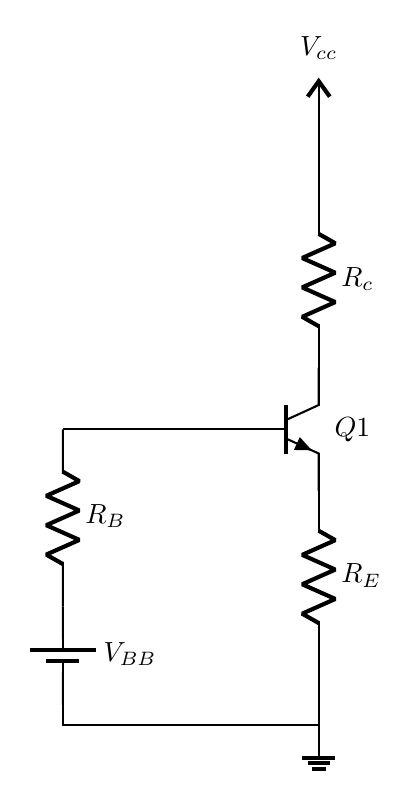
\begin{tikzpicture}
                \node[npn](N1) at (1.59, 2){} node[anchor=west] at (N1.text){$Q1$};
                \draw (1.59, 1.25) to[american resistor, l={$R_E$}] (1.59, -1);
                \draw (1.59, 5.02) to[american resistor, l={$R_c$}] (1.59, 2.77);
                \draw (1.59, -1) -| (1.59, -1.25);
                \node[vcc](N2) at (1.59, 6){} node[anchor=south] at (N2.text){$V_{cc}$};
                \draw (1.59, 5.25) -| (1.59, 6);
                \node[ground] at (1.59, -1.75){};
                \draw (1.59, -1.25) -| (1.59, -1.75);
                \draw (-1.66, 2) to[american resistor, l={$R_B$}] (-1.66, -0.25);
                \draw (-1.66, -0.25) to[battery1, l={$V_{BB}$}] (-1.66, -1.5);
                \draw (-1.66, 2) -| (0.75, 2);
                \draw (-1.66, -1.5) -| (-1.66, -1.75) -- (1.59, -1.75);
                \draw (1.59, 5.02) -| (1.59, 5.25);
            \end{tikzpicture}
            \caption{Malla de entrada simplificada por Thévenin.}
            \label{fig:malla-entrada}
        \end{minipage}%
        \begin{minipage}{0.4\textwidth}
            \centering
            Donde $R_{B}$ la resistencia equivalente y $V_{BB}$ es la tensión de Thévenin:
            \begin{align*}
                R_{B} &= R_1||R_2=\frac{R_1 R_2}{R_1 + R_2} \\
                V_{BB} &= V_{CC} \cdot \frac{R_1}{R_1 + R_2} \\
            \end{align*}
        \end{minipage}
    \end{figure}

    Aplicando LKV a la malla de entrada:

    \begin{align*}
        V_{BB} - I_{BQ} R_B - V_{BEQ} - I_{CQ} R_E &= 0 \\
        V_{BB} - \frac{I_{CQ}}{\beta} R_B - V_{BEQ} - I_{CQ} R_E &= 0 \\
        I_{CQ} &= \frac{V_{BB} - V_{BEQ}}{R_E + \frac{R_B}{\beta}} 
    \end{align*}

Considerando el siguiente criterio de diseño: 

\begin{equation*}
    R_E  \gg \frac{R_b}{\beta} \therefore R_E = 10\frac{R_B}{\beta} \therefore \frac{R_B}{\beta} = \frac{R_E}{10}
\end{equation*}

Se tiene:

\begin{equation*}
    I_{CQ} = \frac{V_{BB} - V_{BEQ}} {R_E + \frac{R_E}{10}}
\end{equation*}


    

\subsection{Teorema de Thévenin en red de entrada}
    \subsection{Análisis de malla de entrada}
    \subsection{Criterios de diseño y fórmulas generales}
    \subsection{Cálculo final de R1 y R2}
  \section{Simulación}
    \subsection{Simulación con valores de diseño}
    \subsection{Simulación con valores normalizados}
    \subsection{Comparación con cálculos analíticos}
  \section{Implementación y mediciones}
    \subsection{Mediciones en circuito implementado}
    \subsection{Consideraciones de medición}
    \subsection{Cálculo de parámetros a partir de mediciones}

\chapter{Análisis y trazado de rectas de carga}
  \section{Recta de carga en corriente continua (CC)}
    \subsection{Ecuación y puntos de corte}
  \section{Recta de carga en corriente alterna (CA)}
    \subsection{Ecuación y puntos de corte}
  \section{Obtención experimental de parámetros}
    \subsection{Corrientes en el divisor resistivo}
    \subsection{Verificación de resultados}

\chapter{Mediciones de pequeña señal}
  \section{Análisis teórico (método analítico)}
    \subsection{Circuito híbrido equivalente}
    \subsection{Cálculo de $Z_i$, $Z_o$, $A_i$ y $A_v$}
  \section{Análisis experimental}
    \subsection{Impedancia de entrada}
    \subsection{Ganancia de tensión}
    \subsection{Ganancia de corriente}
    \subsection{Impedancia de salida}


\end{document}
